%-----------------------------------------------------------------------------%
\chapter{ANALISIS DAN PERANCANGAN SISTEM}
%-----------------------------------------------------------------------------%
\vspace{4.5pt}

Pada bab ini menjelaskan analisis masalah yang diatasi, alur kerja dari perangkat lunak yang dikembangkan, arsitektur dan metode yang digunakan serta hasil evaluasi

\section{Analisis Masalah}
Arsitektur ERP yang digunakan pada Odoo yaitu arsitektur Service Oriented Architecture (SOA) dan masih dideploy secara monolitik, seperti yang sudah dijelaskan pada landasan teori. Arsitektur monolitik memiliki kelemahan dan permasalahan yang bisa diselesaikan dengan arsitektur \textit{microservice}. Aplikasi ERP juga diperlukan untuk memiliki skalabilitas yang baik dan kustomisasi.

Namun untuk melakukan perubahan arsitektur harus dilakukan dekomposisi, proses dekomposisi sendiri tidak mudah karena proses dekomposisi masih membutuhkan analisis secara manual dan untuk mengidentifikasi \textit{service} sulit karena banyaknya pendekatan dan pertimbangan.
Pada penelitian ini menggunakan pendekatan Hierarchical clustering untuk membantu menemukan \textit{service} yang tepat, di mana hierarchical clustering memberikan rekomendasi bagaimana pengelompokan \textit{service} berdasarkan pemilihan partisi terbaik.
Proses dimulai dari melalukan analisis kode seperti Call Graph yang dihasilkan dari kode aplikasi Odoo. Hasil analisis kode di ekstraksi menjadi matrix untuk dilakukan hierarchical clustering. Cluster terbaik dipilih melalui nilai secara struktural yaitu nilai \textit{coupling}  dan \textit{cohesion}.

Hasil terbaik dari clustering diimplementasikan menjadi \textit{service}, penelitian ini akan menggunakan strategi dengan pola \textit{strangle} untuk memecah kode di monolitik. Untuk dekomposisi pada data akan menggunakan strategi \textit{Aggregate Exposing Monolith}.

Microservice yang dibentuk akan dievaluasi melalui uji beban dan penggunaan sumber daya aplikasi untuk menentukan apakah dengan arsitektur \textit{microservice} dapat menyelesaikan permasalahan yang muncul pada arsitektur monolitik di aplikasi ERP.
\\

\section{Kerangka Pemikiran}
\begin{center}
	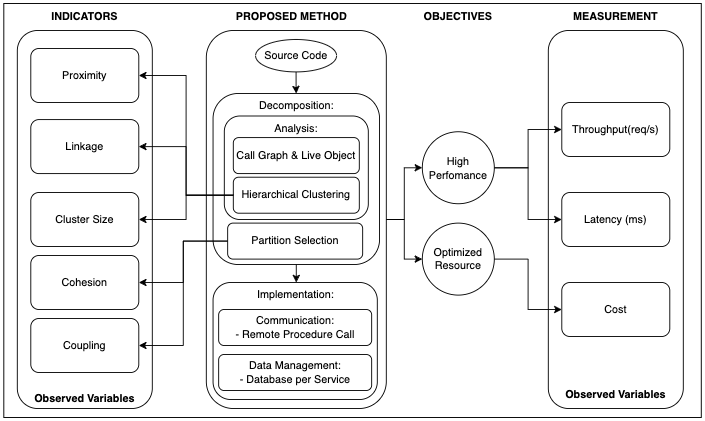
\includegraphics[width=14cm]{img/KerangkaPemikiran.png}
	\captionof{figure}{Kerangka Pemikiran}
	\label{fig:asd}
\end{center}

Penelitian akan dimulai dengan menggunakan kode sumber aplikasi yang dibuat dengan monolitik. Kode sumber dilakukan proses dekomposisi yaitu dengan analisis seperti mencari objek beserta atributnya, untuk mencari keterhubungan lebih lanjut tentang objek maka dilakukan pencarian pada fungsi-fungsi sehingga terbentuklah \textit{call graph} yang menunjukkan bagaimana keterhubungan masing-masing objek di aplikasi.

Dari \textit{graph} yang sudah dibuat akan dilakukan pengelompokan dengan pendekatan Hierarchical Clustering. Di mana perlu ditentukan cara menghitung kedekatan antara objek dan pemilihan algoritma Linkage. Metode linkage yaitu menentukan jarak atau kemiripan antara semua objek. Untuk menentukan jarak ini bisa dengan rata-rata, maximum, dan minimum.

Pengelompokan dari Hierarchical Clustering akan dipilih dengan mencari nilai \textit{cohesion} terendah dan  nilai \textit{coupling} tertinggi. Di mana \textit{coupling} mengevaluasi tingkat ketergantungan langsung dan tidak langsung antar objek. Semakin banyak dua objek menggunakan metode masing-masing semakin mereka menjadi satu kesatuan. Sedangkan  \textit{cohesion} akan mengevaluasi kekuatan interaksi antar objek. Biasanya, dua objek atau lebih menjadi interaktif jika metodenya bekerja pada atribut yang sama.

Ketika analisis dekomposisi sudah selesai dilakukan maka akan dilakukan implementasi berdasarkan pengelompokannya masing-masing yang akan menjadi \textit{service}. Untuk metode komunikasinya antara \textit{service} yaitu dengan Remote Procedure Call(RPC) dan untuk mengelola data, setiap \textit{service} memiliki databasenya masing-masing.

Untuk mengetahui bagaimana performa dari \textit{microservice} dibandingkan dengan monolitik yaitu dengan test beban. Pengukuran performa dilihat dari throughput, jumlah \textit{response}, dan latency. Bagi pengukuran biaya dilakukan melalui menghitung perbandingan antara jumlah sumber daya yang digunakan seperti memori (RAM) dan penggunaan CPU(jumlah core) pada \textit{virtual machine} di masing-masing arsitektur.

\section{Urutan Proses Global}
\begin{center}
	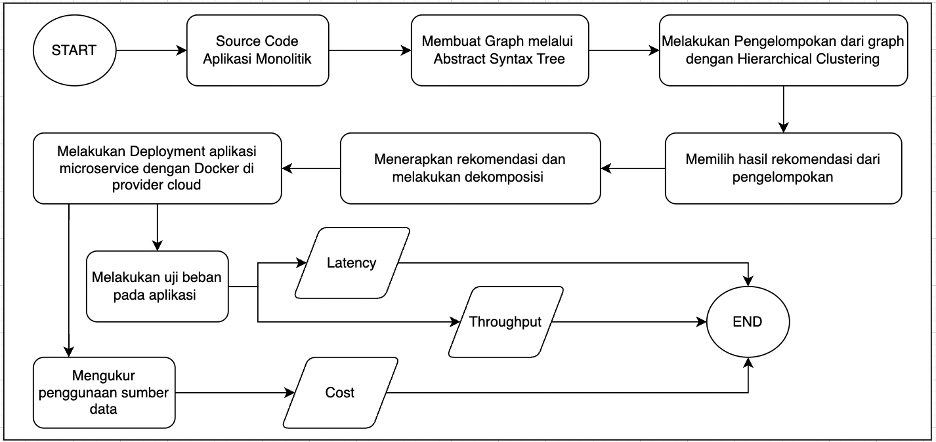
\includegraphics[width=14cm]{img/FlowchartProsesGlobal.png}
	\captionof{figure}{Diagram Flowchart Proses Global }
	\label{fig:asd}
\end{center}

\subsection{Proses Clustering}

\subsubsection{Pengambilan Source Code}
Aplikasi ERP Odoo merupakan aplikasi berlisensi open source, kode program dapat diunduh melalui situs repository Odoo. Pada tugas akhir ini menggunakan Odoo versi 16 dengan status pengujian lulus. Agar kode program dapat berjalan dengan lancar maka diperlukan proses installasi library, module dan Package yang digunakan dari file requirement.txt
\begin{center}
	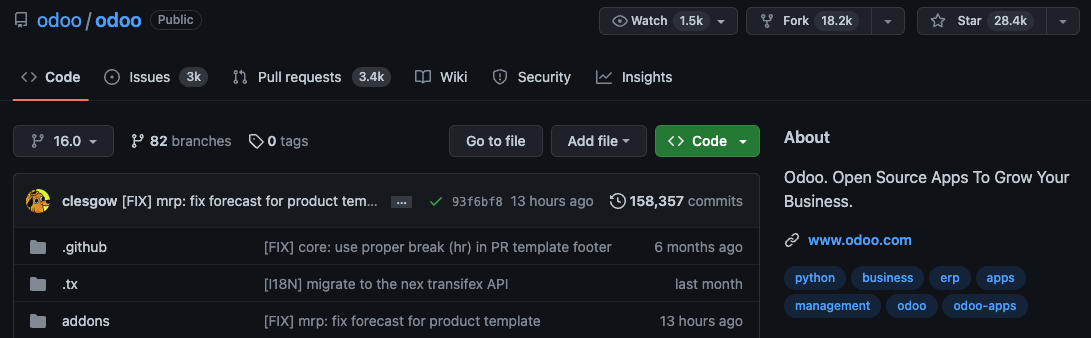
\includegraphics[width=14cm]{img/bab_3/github.png}
	\captionof{figure}{Source Code Aplikasi Odoo pada git repository}
	\label{fig:asd}
\end{center}
\subsubsection{Pembuatan Call Graph}
Pada tugas akhir ini menggunakan tools PyCG untuk menghasilkan \textit{call graph} dalam bentuk format JSON. Terdapat 2 target folder yang dibuat \textit{call graph} yaitu folder odoo.addons dan folder addons karena folder lainnya tidak memiliki hubungan mengenai proses bisnis. Untuk menghemat waktu pembuatan \textit{call graph} maka folder test tidak dibuat.  

\textit{Entry point} untuk \textit{tools} PyCG adalah semua file di target folder dengan ekstensi file .py serta ditentukan package yang ingin diolah menjadi \textit{call graph}. Proses eksekusi dilakukan melalui terminal. Call graph yang dihasilkan berisi \textit{call} yang berasal dari file .py yang ditentukan sebelumnya dan semua module yang terhubungan dari target. Semua module ini bisa diluar dari target module apabila keterhubungan itu terus berlanjut. PyCG hanya bisa menghasilkan \textit{call graph} tanpa informasi mengenai jumlah pemanggilan dan urutan pemanggilan.

\begin{center}
	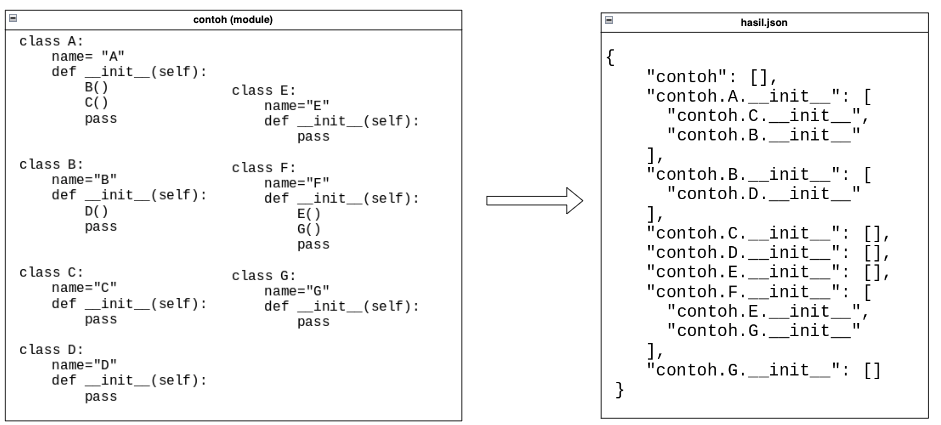
\includegraphics[width=13cm]{img/bab_3/soToCG.png}
	\captionof{figure}{Proses Pembuatan Call Graph dengan PyCG}
	\label{contoh_json_pycg}
\end{center}

Proses ekstraksi json yang dihasilkan dari tools PyCG berupa 2 file JSON masing masing adalah odoo dan addons. Kedua file JSON digabungkan dan menjadi satu \textit{graph} yang direpresentasikan dalam bentuk adjacency list di python.

\subsubsection{Ekstraksi Dependency Module}
Keterbatasannya informasi \textit{call graph} yang dihasilkan dari PyCG, sehingga tugas akhir ini menggunakan library python yaitu 'inspect' untuk menganalisis object secara run-time. Hal ini disebabkan python adalah bahasa pemrogram dinamik di mana pengecekan tipe data dilakukan secara 'run-time'. Ekstrasi ini difokuskan pada module yang memiliki proses bisnis seperti module addons dan odoo/addons. Dari gambar 3.5 bisa diketahui penggunaan inspect bisa menemukan atribut apa saja dan nilainya dari atribut pada objek. 

\begin{center}
	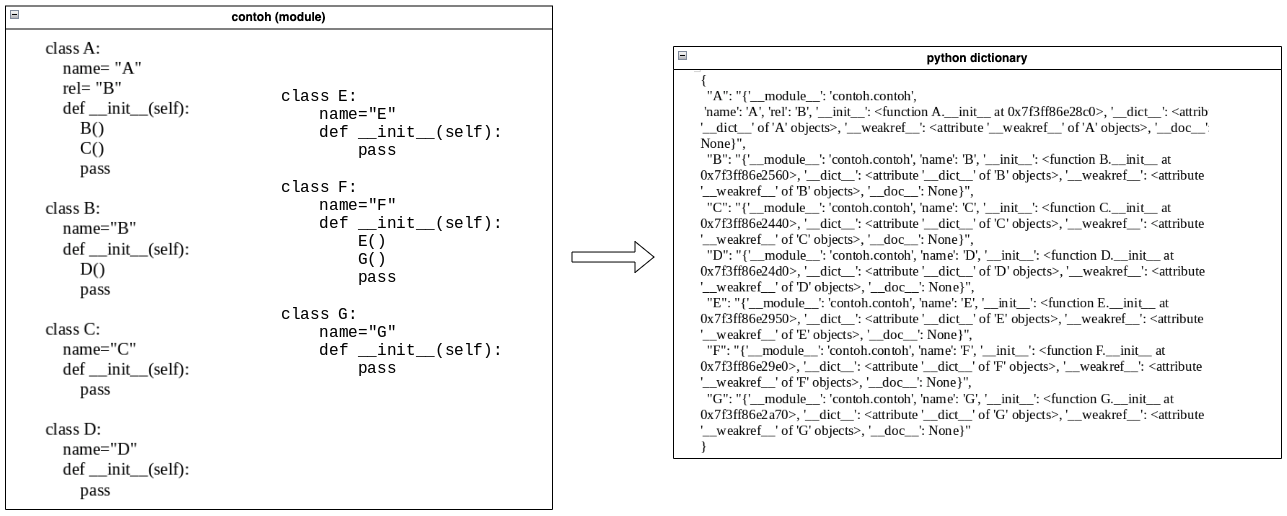
\includegraphics[width=13cm]{img/bab_3/inspectSample.png}
	\captionof{figure}{Penggunaan 'inspect' untuk melihat object python lebih mendalam}
	\label{contoh_json_pycg}
\end{center}

Object yang dianalisis yaitu \textit{class} yang merupakan turunan dari \textit{class} odoo.models.MetaModel, di mana \textit{class} MetaModel memiliki properti seperti  name, \_inherits , \_inherit, dan attribute\_rel. Hasil ekstrasi depedency module digabungkan melalui nama module PyCG 
\\
\subsubsection{Pengabungan dan Optimisasi Hasil Ekstraksi}
Graph yang dihasilkan dari proses ekstrasi dipisahkan antara module eksternal dan module internal. Module yang digunakan untuk pengelompokan adalah module internal, setiap \textit{call} yang dilakukan memiliki nama \textit{call} yang berupa gabungan antara nama fungsi / \textit{class} / module /file di kode program. PyCG tidak memberikan informasi apakah nama \textit{call} tersebut berupa tipe apa, untuk itu pengelompokan dilakukan secara hybrid yaitu berdasarkan module dan file. 

Nama \textit{call} yang disatukan menjadi module adalah \textit{call} yang memiliki awalan(root) addons atau odoo/addons dan nama \textit{call} yang disatukan dengan file adalah nama \textit{call} selain addons. Call yang dikelompokkan memiliki nilai agregasi dari jumlah \textit{call}. Jumlah \textit{call} dapat digunakan sebagai weight yang dapat menunjukkan kekuatan antara \textit{call} satu sama lain, proses ini membentuk \textit{call} baru yang lebih ringkas dan relevan dalam bentuk \textit{graph}. 

\subsubsection{Hierarchical Clustering}
Graph yang berbentuk Adjacency list diubah menjadi adjacency matrix, proses normalisasi data dilakukan pada matrix. Tujuan normalisasi data agar nilai \textit{weight}(jumlah \textit{call}) dari relasi berkisar dari 1 hingga 0. Semakin banyak jumlah \textit{call} dilakukan maka nilai mendekati 1,kemudian matrix tersebut dibuat menjadi Distance Matrix, rumus jarak yang digunakan ada 2 yaitu Jaccard dan Struktural Similarity. Masing-masing hasil jarak disatukan dengan rata-rata. Jaccard menghasilkan hasil yang bagus pada remodularisasi perangkat lunak dan Struktural Similarity digunakan untuk melihat kedekatan dari sisi intesitas panggilan antara module.

\begin{center}
	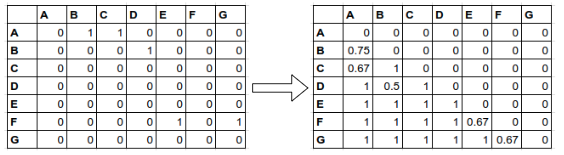
\includegraphics[width=12cm]{img/bab_3/simJaccard.png}
	\captionof{figure}{Perhitungan Jarak Jaccard}
	\label{fig:asd}
\end{center}
\begin{center}
	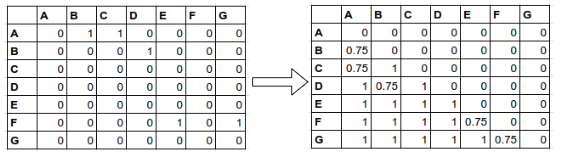
\includegraphics[width=12cm]{img/bab_3/simStr.png}
	\captionof{figure}{Perhitungan Jarak Struktural}
	\label{fig:asd}
\end{center}

\begin{center}
	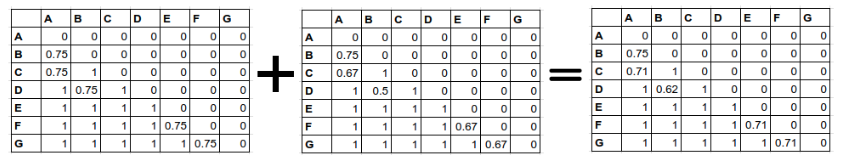
\includegraphics[width=14cm]{img/bab_3/hasilJarak.png}
	\captionof{figure}{Hasil Akhir Jarak}
	\label{fig:asd}
\end{center}
Distance Matrix / Matrix kedekatan dapat dilihat nilai dengan ilustrasi Heatmap, di mana sumbu x dan y adalah semua module dan nilai kedekatannya dengan module lainnya. Semakin terang warna menunjukkan hubungan yang kuat antara module, perlu diketahui bahwa distance matrix merupakan matrix segitiga. Pada tugas akhir ini menggunakan library SciPy untuk melakukan proses \textit{clustering} yang memiliki fungsi Hierarchical Clustering.

\begin{center}
	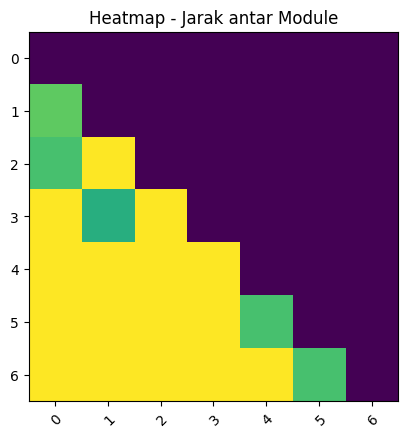
\includegraphics[width=7cm]{img/bab_3/heatmap.png}
	\captionof{figure}{Heatmap yang dihasilkan dari Distance Matrix}
	\label{fig:asd}
\end{center}

Pemilihan pengelompokan dengan hierarchical agglomerative clustering dibandingkan Paritition clustering karena tidak mudah untuk mengetahui jumlah ideal \textit{cluster}. Untuk menentukan metode \textit{linkage} tugas akhir ini menggunakan single lingkage, average linkage, dan complete lingkage. Hasil dari masing-masing lingkage dipilih jumlah partisi yang ideal untuk \textit{microservice}. Penggunaan single lingkage memiliki kecenderungan menghasilkan banyak partisi yang berisi modul sedikit tetapi ada satu partisi memiliki banyak module sedangkan complete linkage menghasilkan partisi yang memiliki jumlah modul yang sama dengan partisi lainnya. Untuk Average lingkage menghasilkan bentuk partisi di antara complete lingkage dan single lingkage.

Hasil pengelompokan dapat ditampilan dalam bentuk dendogram.  Di mana pengelompokan dari setiap linkage memiliki dampak berbeda yang bisa dilihat dari bentuk dan nilai kedekatan antar partisi melalui dendogram dan bentuk relasi. Warna pada garis keterhubungan module memiliki arti sebagai partisi tersendiri karena memiliki jarak yang jauh dari partisi lainnya. 
\begin{center}
	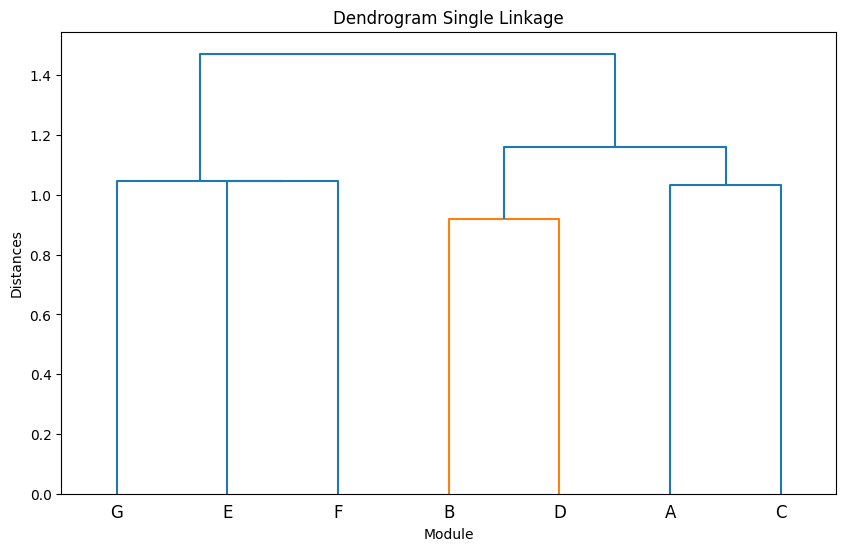
\includegraphics[width=9cm]{img/bab_3/singleLink.png}
	\captionof{figure}{Dendogram Single Linkage}
	\label{fig:asd}
\end{center}
\begin{center}
	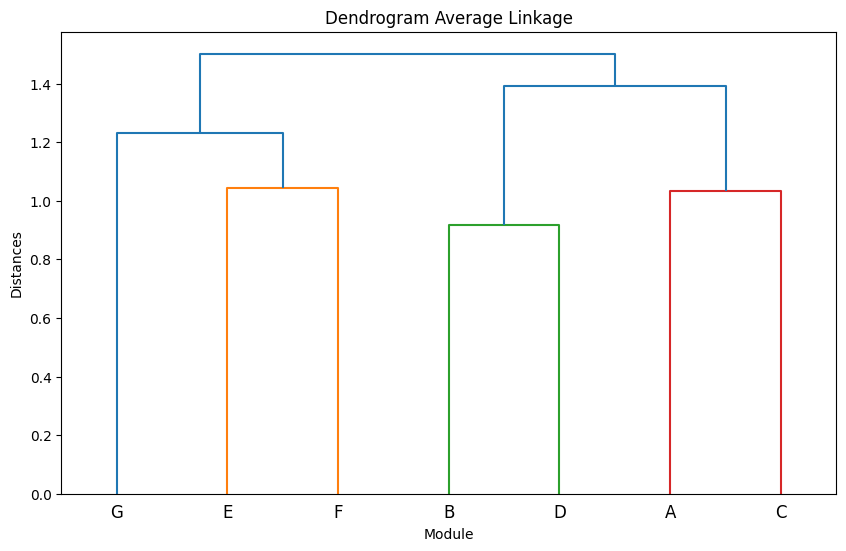
\includegraphics[width=9cm]{img/bab_3/averageLink.png}
	\captionof{figure}{Dendogram Average Linkage}
	\label{fig:asd}
\end{center}
\begin{center}
	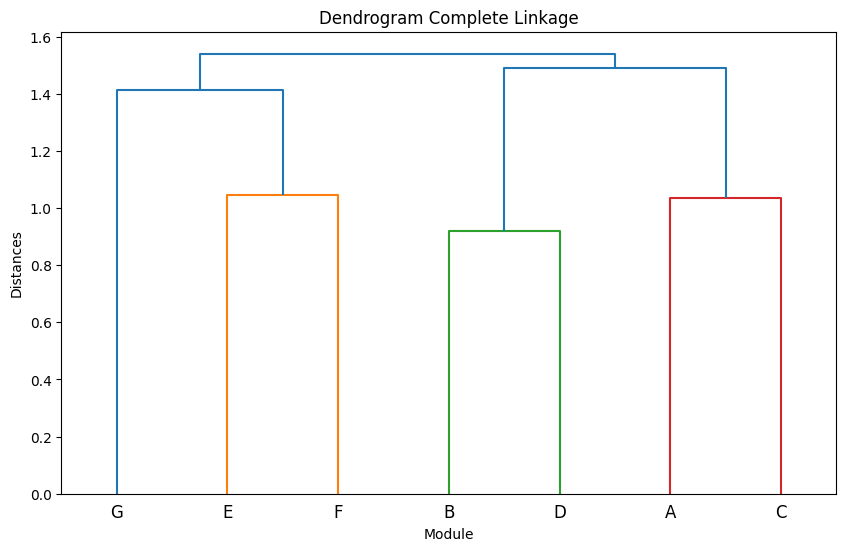
\includegraphics[width=9cm]{img/bab_3/completeLink.png}
	\captionof{figure}{Dendogram Complete Linkage}
	\label{fig:asd}
\end{center}

\subsubsection{Pemilihan Partisi}
Pemilihan jumlah partisi perlu dilakukan dengan perhitungan yang dapat menentukan jumlah \textit{service} yang ideal. Microservice yang ideal memiliki nilai \textit{coupling} yang rendah dan nilai \textit{cohesion} yang tinggi. Untuk itu tugas akhir ini menentukan partisi dengan nilai struktural yang menggunakan persamaan 2.2 dan tidak memperhitungkan nilai \textit{coupling} external karena addons pada Odoo dibuat dengan framework Odoo. Hubungan module luar seperti library umumnya dilakukan oleh framework Odoo sendiri bukan oleh addons.

Untuk pemilihan partisi harus mempertimbangkan nilai \textit{cohesion}, nilai \textit{coupling}, jumlah \textit{service}, dan apakah \textit{service} tersebut seimbang. Partisi yang akan menjadi \textit{service} diharapkan bisa independen. 

Berikut adalah hasil nilai \textit{coupling} dan \textit{cohesion} masing-masing jumlah \textit{cluster}. Semakin tinggi jumlah \textit{cluster} maka nilai \textit{coupling} akan meningkat dan begitu pula sebaliknya untuk nilai \textit{cohesion}. Dari contoh data ditemukan bahwa \textit{cluster} yang ideal berjumlah 2 \textit{service}, karena ketika semakin banyak jumlah \textit{service} maka nilai \textit{coupling} meningkat dan sebaliknya nilai \textit{cohesion} menurun.

\begin{center}
	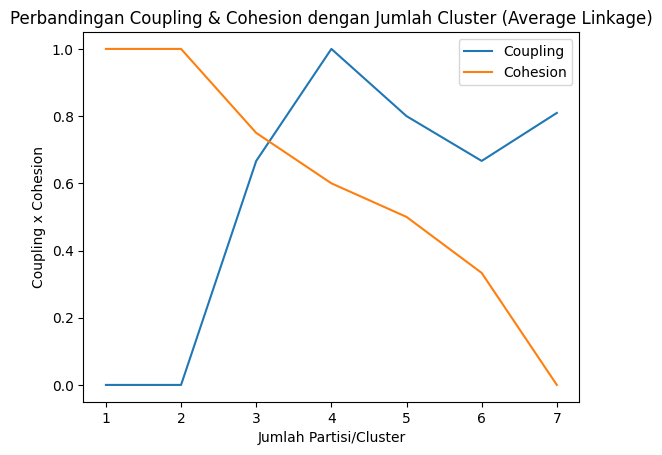
\includegraphics[width=14cm]{img/bab_3/cohVScoup.png}
	\captionof{figure}{Perbandingan dari nilai Cohesion dan nilai Coupling dengan jumlah \textit{cluster}/partisi}
	\label{fig:asd}
\end{center}


\subsection{Dekomposisi Monolitik ke Microservice}
\subsubsection{Pemisahan User Interface}
Odoo adalah aplikasi ERP berbasis web, tampilan pada Odoo bisa dibuka pada broser yang kompatibel. Odoo menggunakan pendekatan SPA (Single Page Application) dan adanya server rendering untuk menghasilkan HTML. UI dapat memanggil API yang berada pada server yang sama, sehingga diperlukan pemisahan kepentingan. Benefit dari proses ini dapat meningkatan skalabilitas dan pengembangan bisa dilakukan secara independen.
\begin{center}
	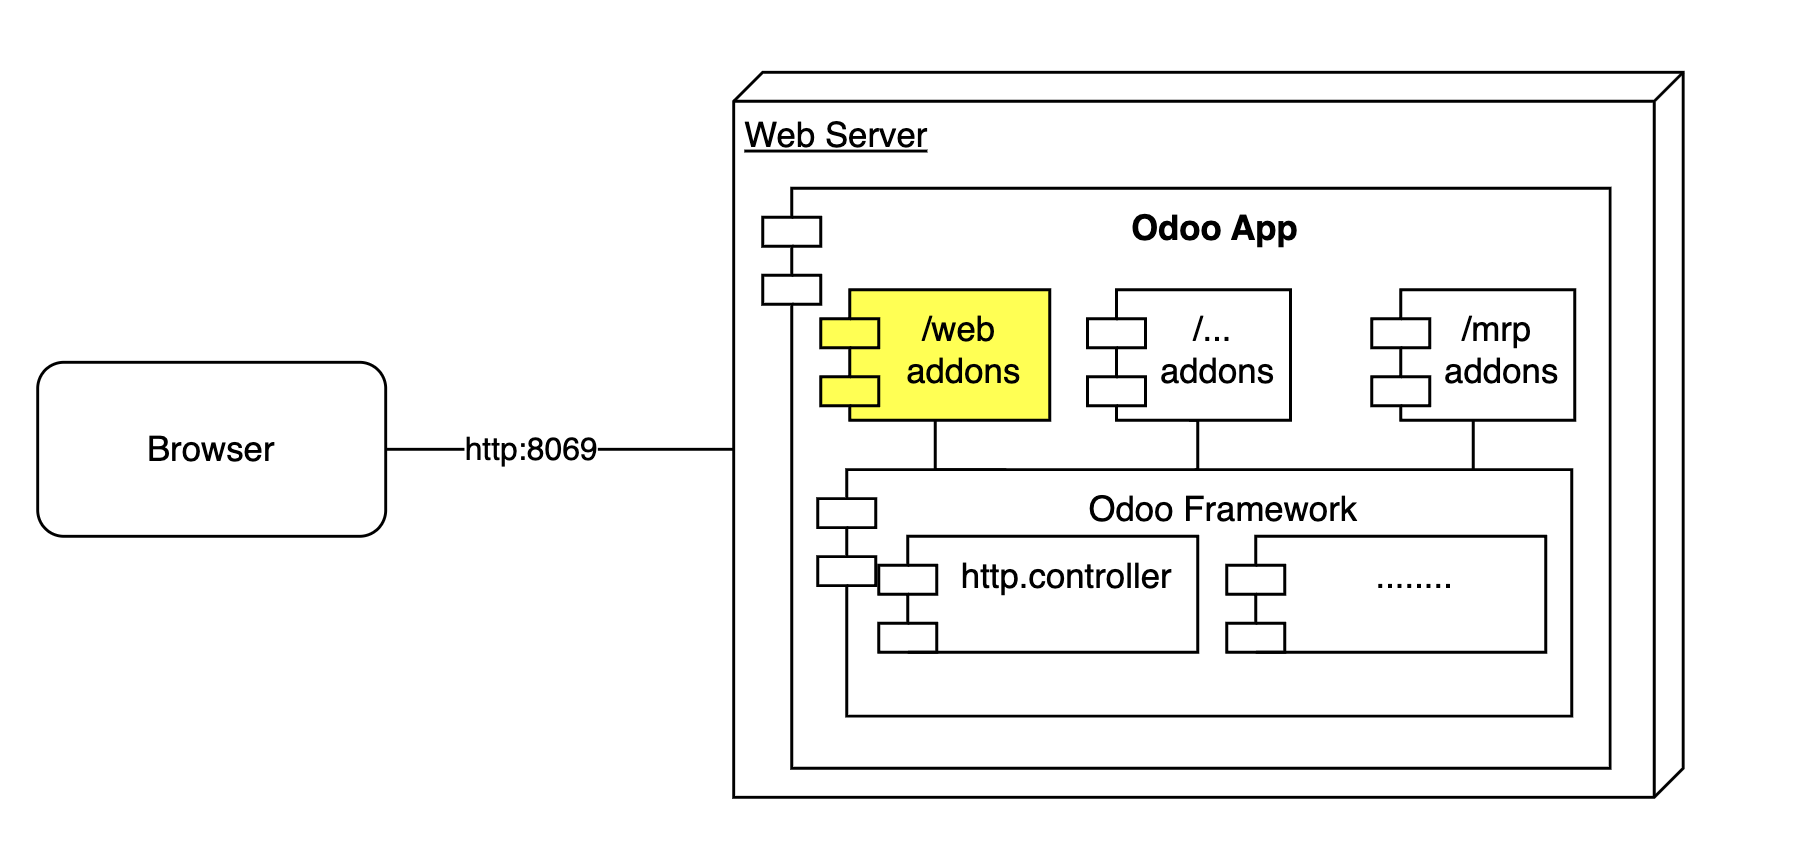
\includegraphics[width=14cm]{img/bab_3/monoUI.png}
	\captionof{figure}{Arsitektur UI Monolitik}
	\label{fig:asd}
\end{center}
Proses pemisahan membutuhkan \textit{reverse} \textit{proxy} yang dapat menghubungkan web server di mana bertanggung jawab pada hal seperti file static(css,js,gambar) dan UI dengan web server lainnya. Tujuan adanya \textit{reverse} \textit{proxy} agar \textit{client} hanya perlu mengetahui satu pintu masuk aplikasi yaitu \textit{reverse} \textit{proxy} itu sendiri dan tidak perlu mengetahui seluruh server yang ada di aplikasi.
\begin{center}
	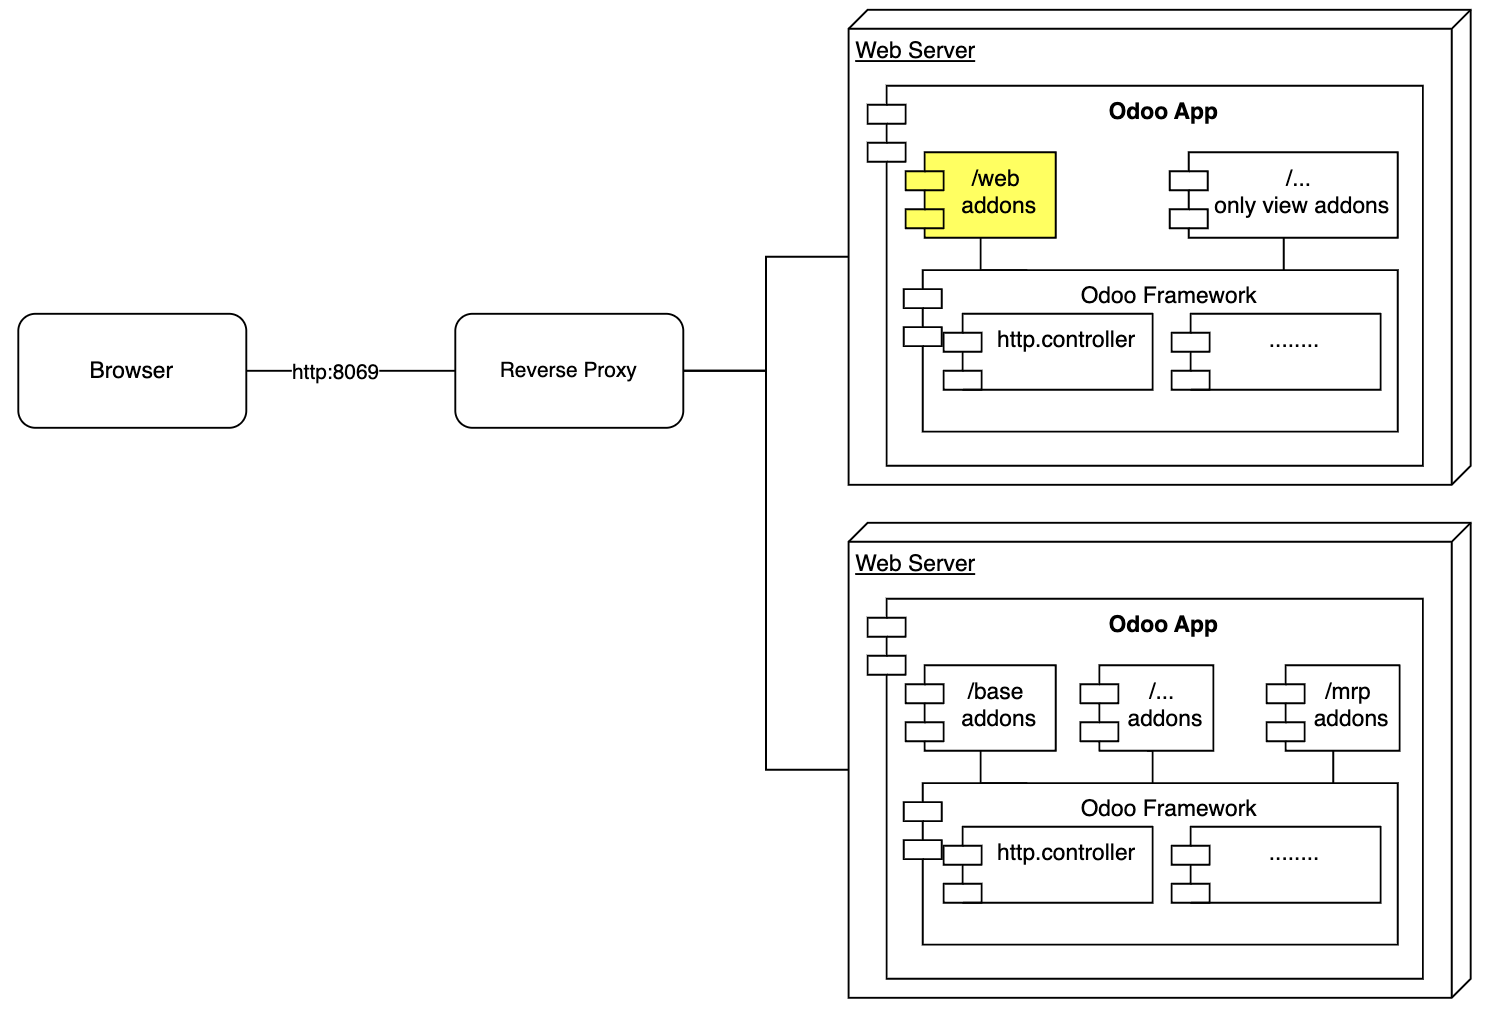
\includegraphics[width=14cm]{img/bab_3/microUI.png}
	\captionof{figure}{Arsitektur UI di Microservice}
	\label{fig:asd}
\end{center}

\subsubsection{Strategi Pemisahan Kode}
Berdasarkan landasan teori terdapat beberapa strategi pemisahan kode aplikasi monolitik, pada tugas akhir ini akan menggunakan 2 strategi yaitu pola \textit{Strangle} dan pola Branch by Abstraction. Pola \textit{Strangle} diterapkan karena pendekatan ini umum diterapkan dan lebih mudah pada suatu aplikasi yang sudah besar, dengan pola ini aplikasi monolitik bisa berdiri bersamaan dengan \textit{service} yang ingin dibangun atau dimigrasi. 

\begin{center}
	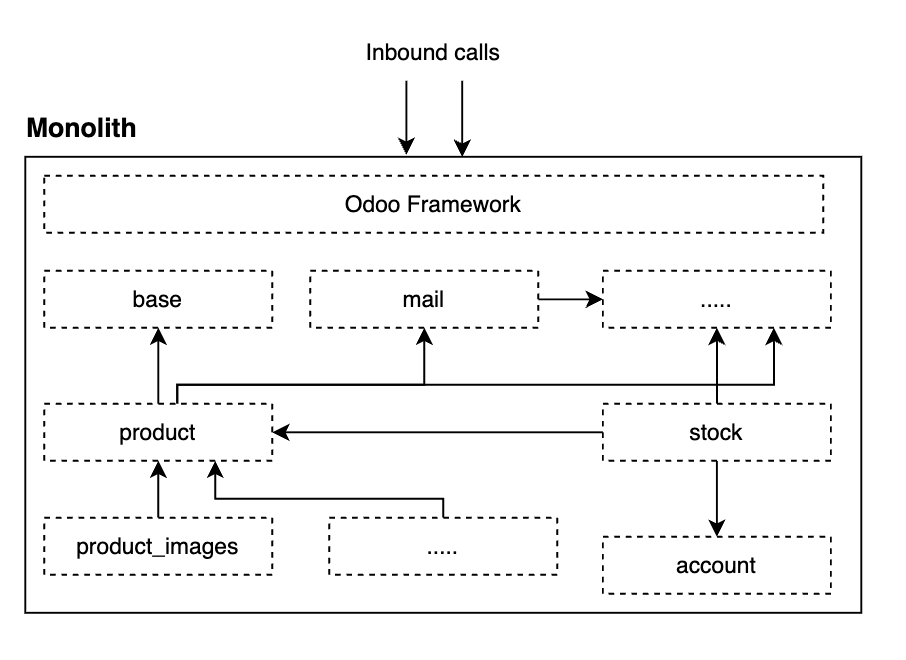
\includegraphics[width=14cm]{img/bab_3/strangelExMono.png}
	\captionof{figure}{Struktur Module dan Keterhubungannya di Aplikasi Monolitik}
	\label{fig:asd}
\end{center}

Terdapat 3 langkah utama dalam menerapkan pola \textit{strangle} yaitu memilih bagian yang ingin dipindahkan, memindahkan aplikasi menjadi \textit{service} yang berdiri sendiri, dan yang terakhir mengubah \textit{call} dari monolitik ke \textit{service} yang baru dibuat. Tugas akhir ini milih bagian yang dipindahkan pada kasus bisnis yaitu 'Product', Product bisa dilakukan penambahan Product baru, perubahan atributnya, pencarian atau mendapatkan product dan penghapusan product.

Proses pemindahan module dibantu dengan hasil clustering yang sudah diproses sebelumnya sehingga dibuat untuk membuat \textit{microservice}. Untuk menghubungkan antara bagian yang sudah dipisah dari monolitik dengan bagian yang masih di monolitik maka diperlukan penerapan pola Branch by Abstraction. Terdapat dua bagian utama yaitu abstract dan adapter. Abstract berperan menggantikan bagian yang sudah pisah menjadi \textit{service} sehingga bagian lain di monolitik tidak terdampak dan Adapter adalah implementasi sesungguhnya yang menghubungkan antara \textit{service} dan aplikasi monolitik.

\begin{center}
	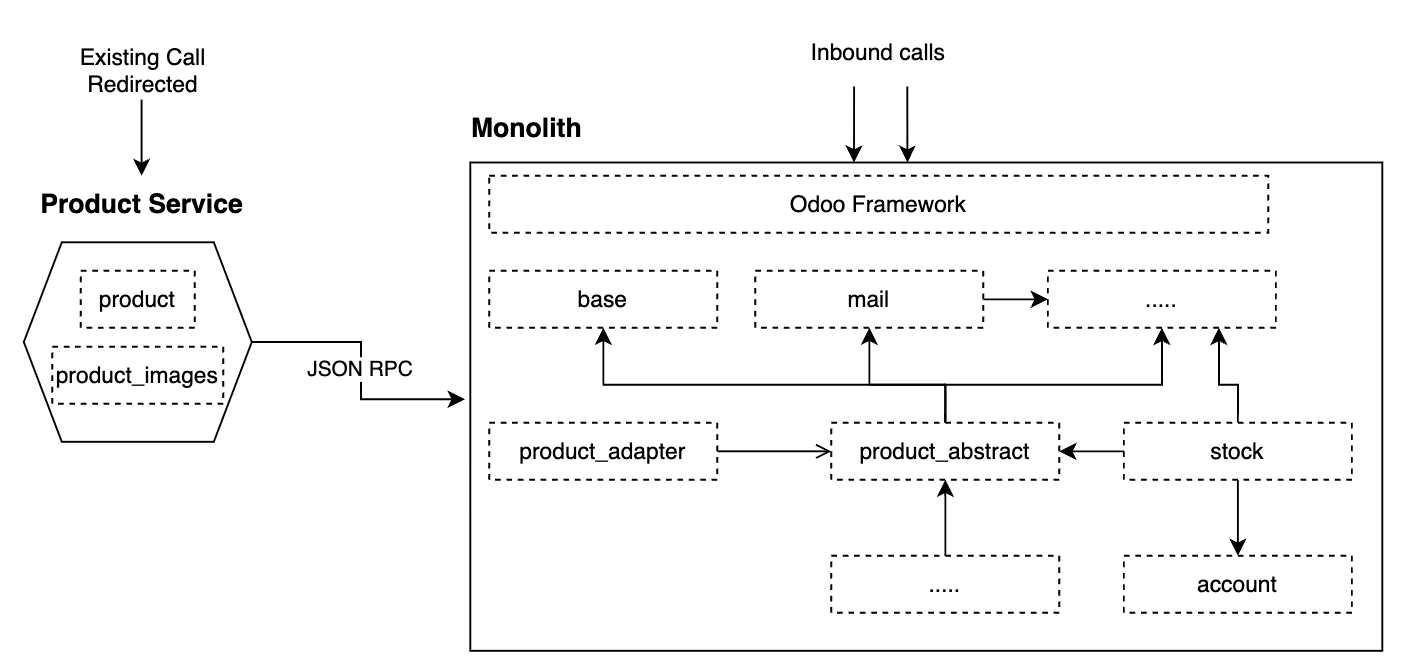
\includegraphics[width=14cm]{img/bab_3/strangelExMicro.png}
	\captionof{figure}{Penerapan Pola \textit{Strangle} dan Branch by Abstraction}
	\label{fig:asd}
\end{center}

Pemisahan kode mempengaruhi proses autentikasi, proses autentikasi pada aplikasi Odoo terdapat 2 cara yaitu melalui password atau API-Key. Odoo menyimpan sesi autentikasi di cookie namun bukan dalam format JWT tapi bentuk HTTP session. Untuk itu diperlukan modifikasi pada sistem autentikasi yang menggunakan format JWT agar setiap \textit{service} tidak perlu menvalidasi berkali-kali apakah sesi itu valid. 

\begin{center}
	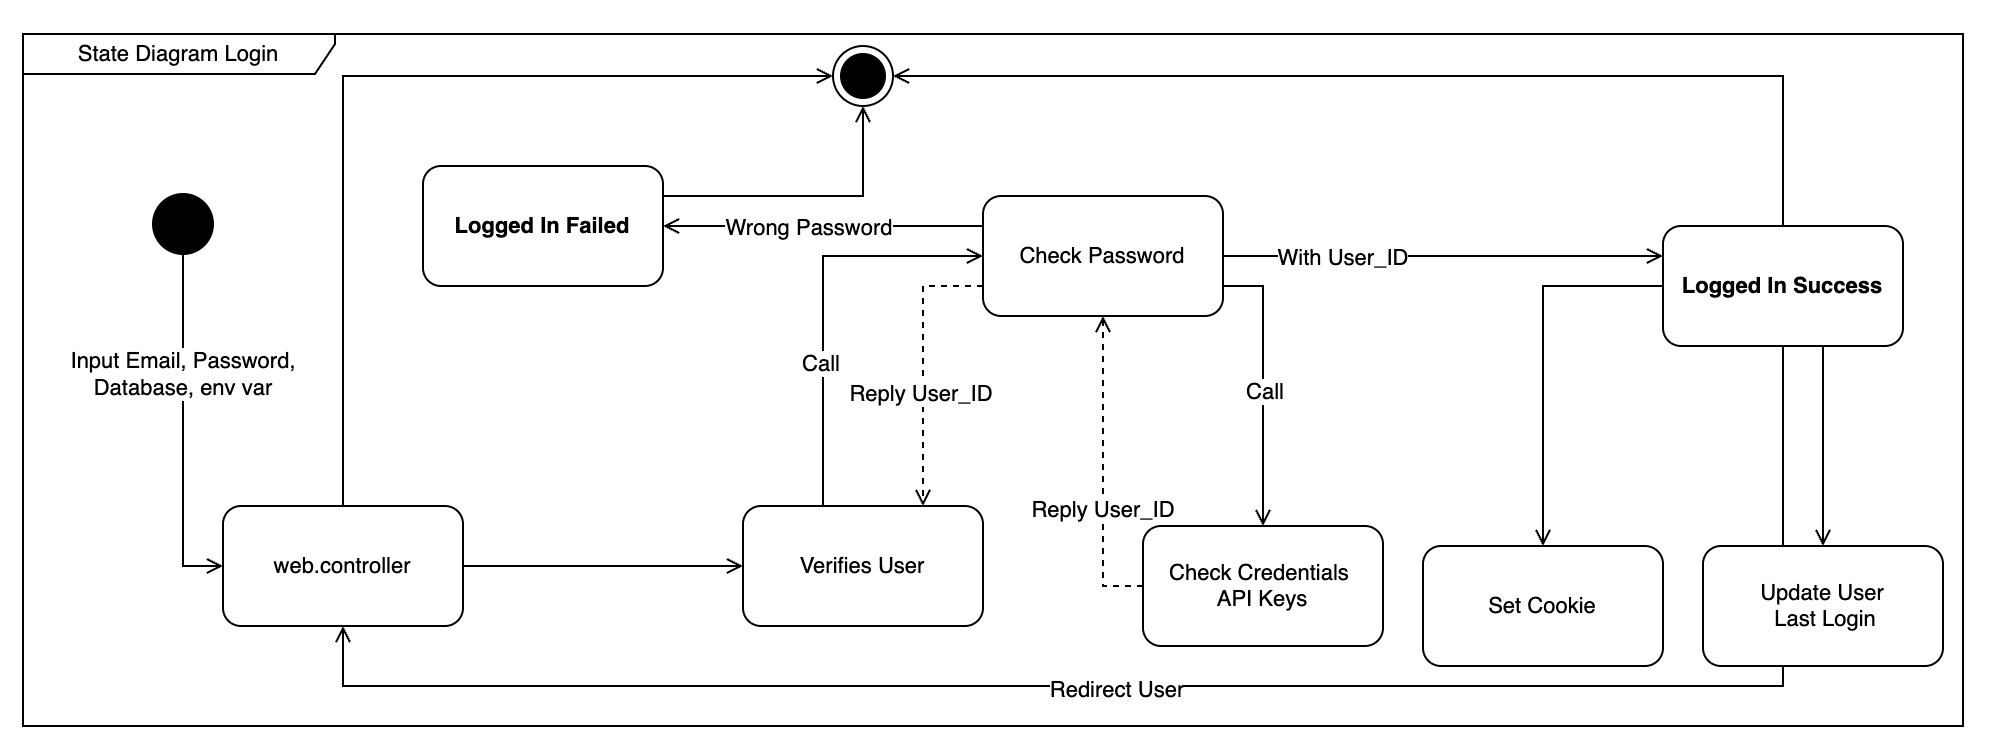
\includegraphics[width=14cm]{img/bab_3/stateDiagramLogin.png}
	\captionof{figure}{State Diagram pada proses login}
	\label{fig:asd}
\end{center}

Pada kasus bisnis untuk mendapatkan product, Odoo memiliki model framework yang memiliki fitur Object Relational Mapping(ORM), fitur controller dan fitur lainnya. Model framework diterapkan pada module addons ataupun odoo.addons, penggunaan model framework masih menjadi satu pada repo sehingga perubahan model dapat menyebabkan kerusakan di bagian addons lainnya. Model framework ini bisa diubah menjadi \textit{shared library} dan menjadi bentuk \textit{microservice chasis}.\\

\begin{center}
	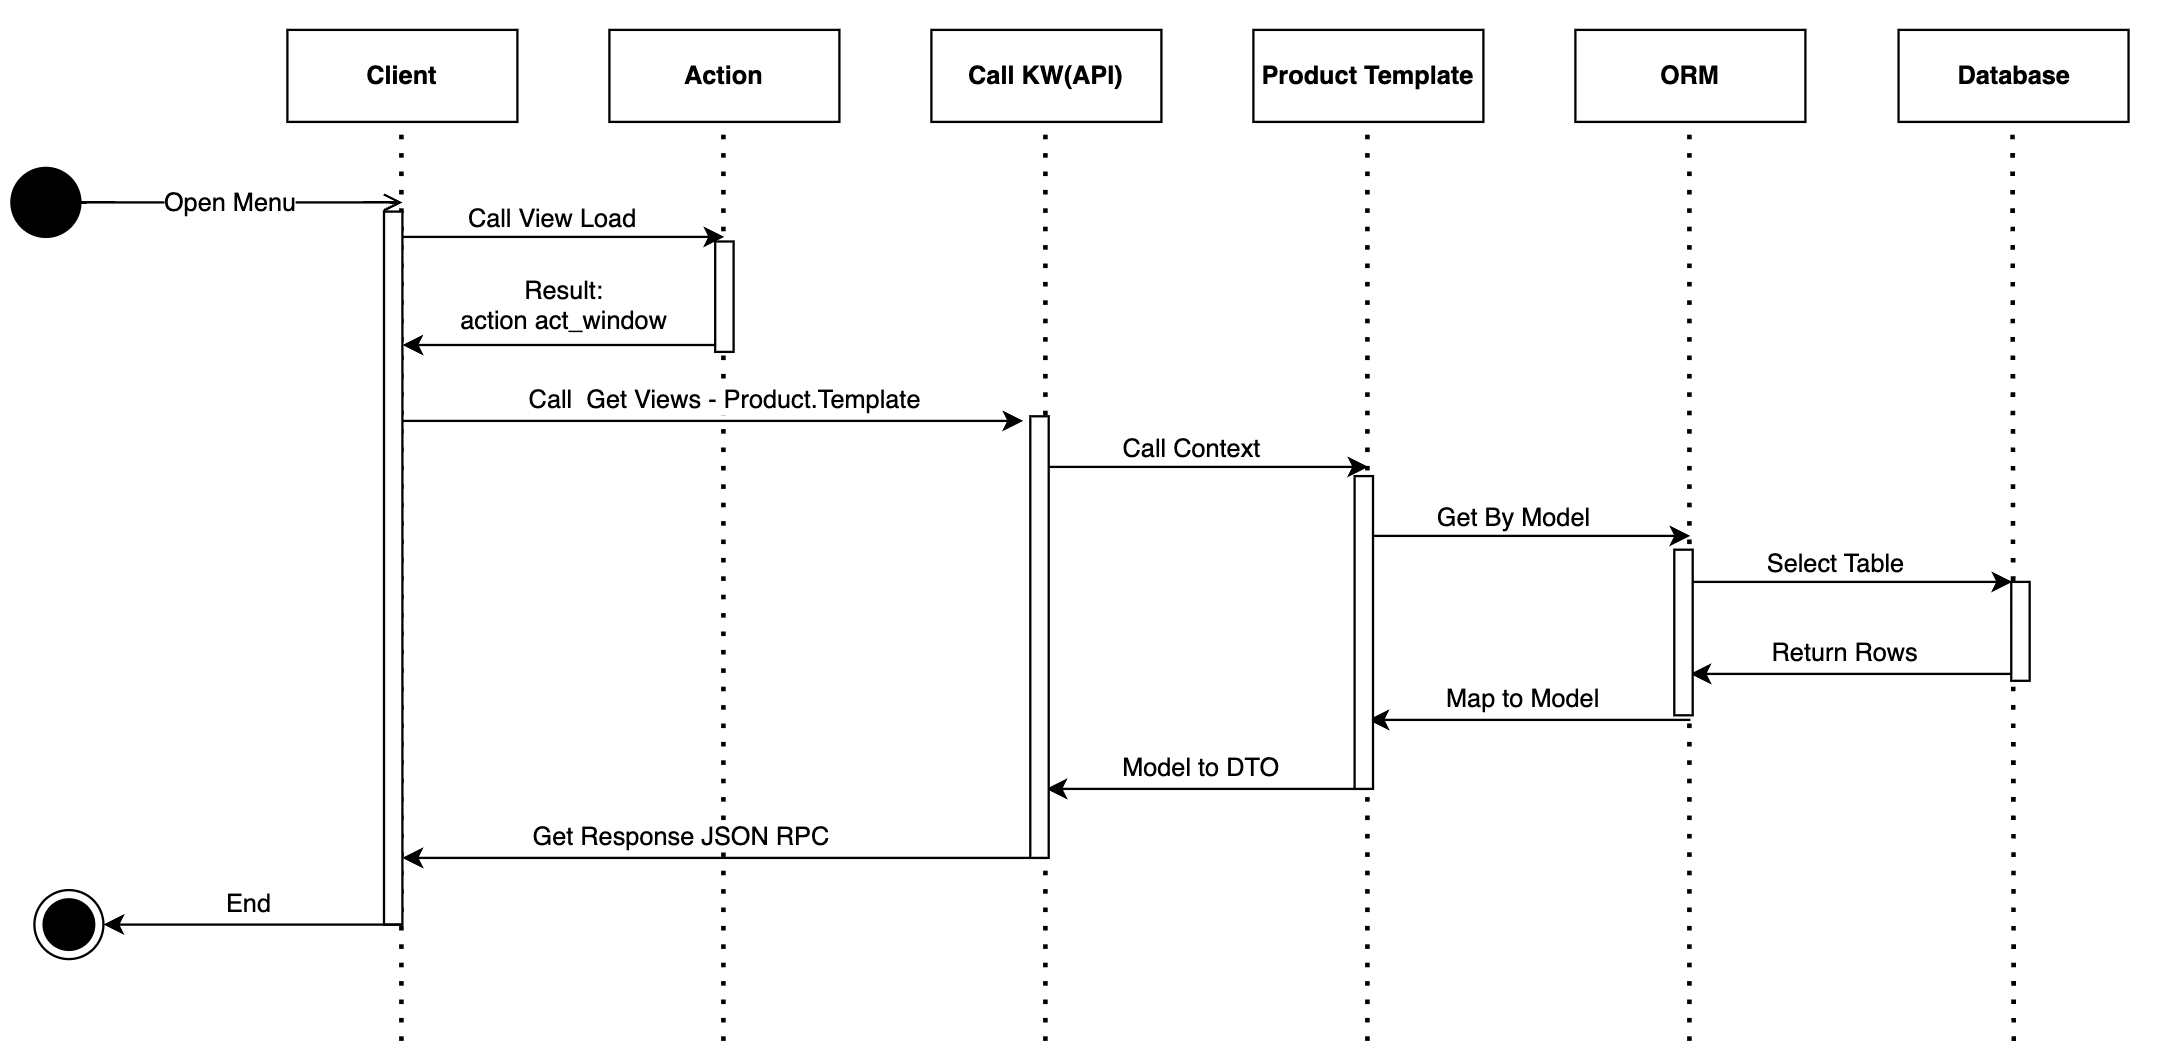
\includegraphics[width=14cm]{img/bab_3/seqDiagGet.png}
	\captionof{figure}{Sequence Diagram pada kasus pengambilan data Product}
	\label{fig:asd}
\end{center}
\subsubsection{Komunikasi antar service}
Proses komunikasi antar \textit{service} dilakukan melalui JSON-RPC karena Odoo sudah memiliki untuk setiap addonsnya RPC ini bisa berupa XML atau JSON. Apabila diperlukan penambahan metode komunikasi lainnya seperti gRPC maka harus dibangun \textit{service} yang mengubah gRPC menjadi JSON-RPC atau sebaliknya.  
\\
\subsubsection{Strategi Pemisahan \textit{database}}
Pemisahan \textit{database} dilakukan setelah dilakukan pemisahan kode karena pada Odoo sudah terdapat ORM yang mengelola \textit{database}. Ketika \textit{database} ingin dipisahkan maka pengaksesan \textit{database} monolitik  digunakan sebagai data access layer melalui API yang bisa berupa JSON-RPC.
\\
\subsection{\textit{Deployment}}
\begin{center}
	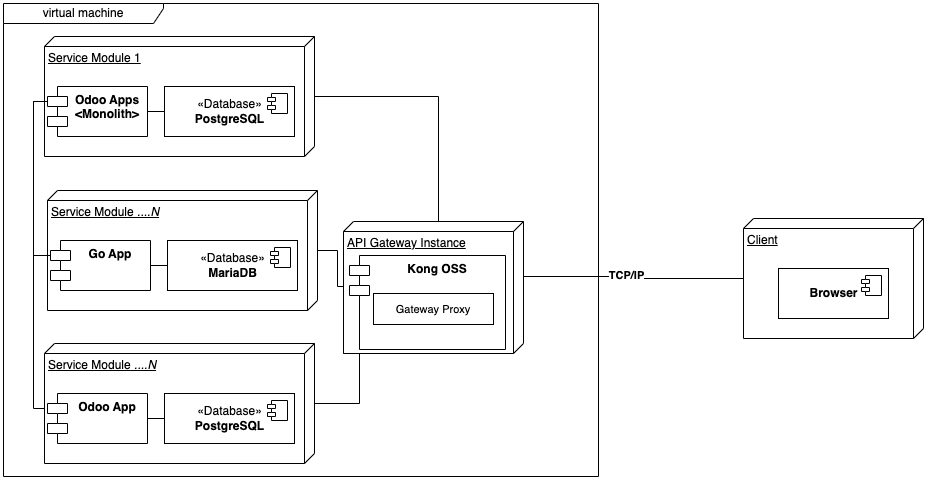
\includegraphics[width=14cm]{img/bab_3/Deployment.png}
	\captionof{figure}{Diagram \textit{Deployment}}
	\label{fig:asd}
\end{center}
Pendekatan \textit{Deployment} Service yang digunakan adalah pola \textit{container} karena \textit{container} memiliki proses\textit{deployment} yang ringan dan modern. Container ini bisa dijalankan melalui Virtual Machine atau langsung dari host, selain itu \textit{container} memiliki banyak keuntungan seperti mengenkapsulasi teknologi, setiap server instance terisolasi, performa juga tidak buruk.  

Tugas Akhir ini menggunakan \textit{API Gateway} Kong \textit{(off-the-shelf)} karena Kong sudah memiliki fitur yang lengkap pada kasus migrasi aplikasi monolitik ke \textit{microservice}. Fitur itu berupa kemampuan untuk redireksi url untuk menerapkan proses \textit{strangle}, pemantauan \textit{service}, dan memiliki performa yang baik.
